% Pour les réfractaires de LaTex, ce rapport s'édite très bien en ligne sur https://www.overleaf.com

\documentclass[11pt]{article}

% Character set for input and output
\usepackage[utf8]{inputenc}
\usepackage[T1]{fontenc}
\usepackage[english,french]{babel}

% Fonts
\usepackage{libertine}
\usepackage[scaled=0.83]{beramono}

% AMS math-packages
\usepackage{amssymb}
\usepackage{amsmath,amsthm}

% TODO in text
\usepackage{todonotes}

% URL (clickable), references within document, etc./
\usepackage{hyperref}

% Code formatting
\usepackage{listings}
\lstset{
   language=java,
   extendedchars=true,
   basicstyle=\footnotesize\ttfamily,
   showstringspaces=false,
   showspaces=false,
   numbers=left,
   numberstyle=\footnotesize,
   numbersep=9pt,
   tabsize=2,
   breaklines=true,
   showtabs=false,
   frame=single,
   extendedchars=false,
   inputencoding=utf8,
   captionpos=b
}

% Text / Paragraph space
\addtolength{\textwidth}{1.5cm}
\addtolength{\hoffset}{-0.5cm}
\setlength{\parindent}{0pt}
\setlength{\parskip}{1.5ex plus 1ex minus 1ex}

\title{\'Evaluation de performances\\ de programmes multi-threadés}
\author{{\Large Group ...}\\
\quad NOM Prénom 1 \quad NOM Prénom 2 \\{...,...}@etu.univ-grenoble-alpes.fr}
\date{\today{}}
%\date{December 14, 2022}

\begin{document}

\maketitle

\section*{Introduction}
%
Ce rapport présente notre travail d'expérimentation sur le TP d'évaluation de performances. Nous avons 

... ce que vous avez réussi à faire ...

\todo{Ceci est un exemple...}
\begin{itemize}
\item
  Nous avons effectué toutes les expérimentations.
\item
  Avons trouvé la meilleure valeur de nombre de threads pour les configurations concernées. 
\item
  Avons effectué les expérimentations sur un portable personnel, en local sur les macines de l'UFR et sur le serveur mandelbrot. 
\end{itemize}

... ce que vous n'avez pas fait ...


... les analyses que vous avez pu mener ...

... ce que vous en avez pensé/apprécié/dur/...
%


\section{Utilisation des fonctions \texttt{gettimeofday} et \texttt{getrusage}}

Rappeler la différence entre les deux.

Dire laquelle vous avez utilisé pour les mesures d'accélération.

Spécifier où vous avez placé les appels. Mettre du code pour illustrer ici ou en annexe.

Exemple de listing de code.
\begin{lstlisting}[language=C]
int main(int argc, char *argv[]) {
    ...
    /* Algo */
	gettimeofday(&t1,NULL);    
    algo_principal(parallelism, tableau, taille, arg);
    gettimeofday(&t2,NULL);
    ...
}    
\end{lstlisting}

%%%%%%%%%%%%%%%%%%%%%%%%%%%%%%%%%%%%%%
\section{Expérimentation}

\subsection{Configurations matérielles}

Spécifier les machines sur lesquelles vous avez travaillé. Il faut donner le nombre de CPU/threads, mémoire, disque. Ainsi que la version du système (Linux ...) et de gcc.

Exemple : Nous avons effectué nos mesures sur un MacBook Pro 16 pouces avec 1 CPU 2,3 GHz Intel Core i9 à 8 cœurs et 32 Go 2667 MHz DDR4 de mémoire. Le système et MacOS 11.7 et la compilation est faite avec Apple clang version 13.0.0.

\subsection{Configurations}

... Tailles de vecteurs considérées ...

... Nb de threads considérés ...


\subsection{Accélération dans le cas de vecteurs de petite taille}

Détailler l'étude du speedup en fonction du nb de threads pour la petite taille.

Vous devez inclure ici un graphique de ce type et commenter.

\begin{figure}[ht]
\label{fig:t1}
\centering
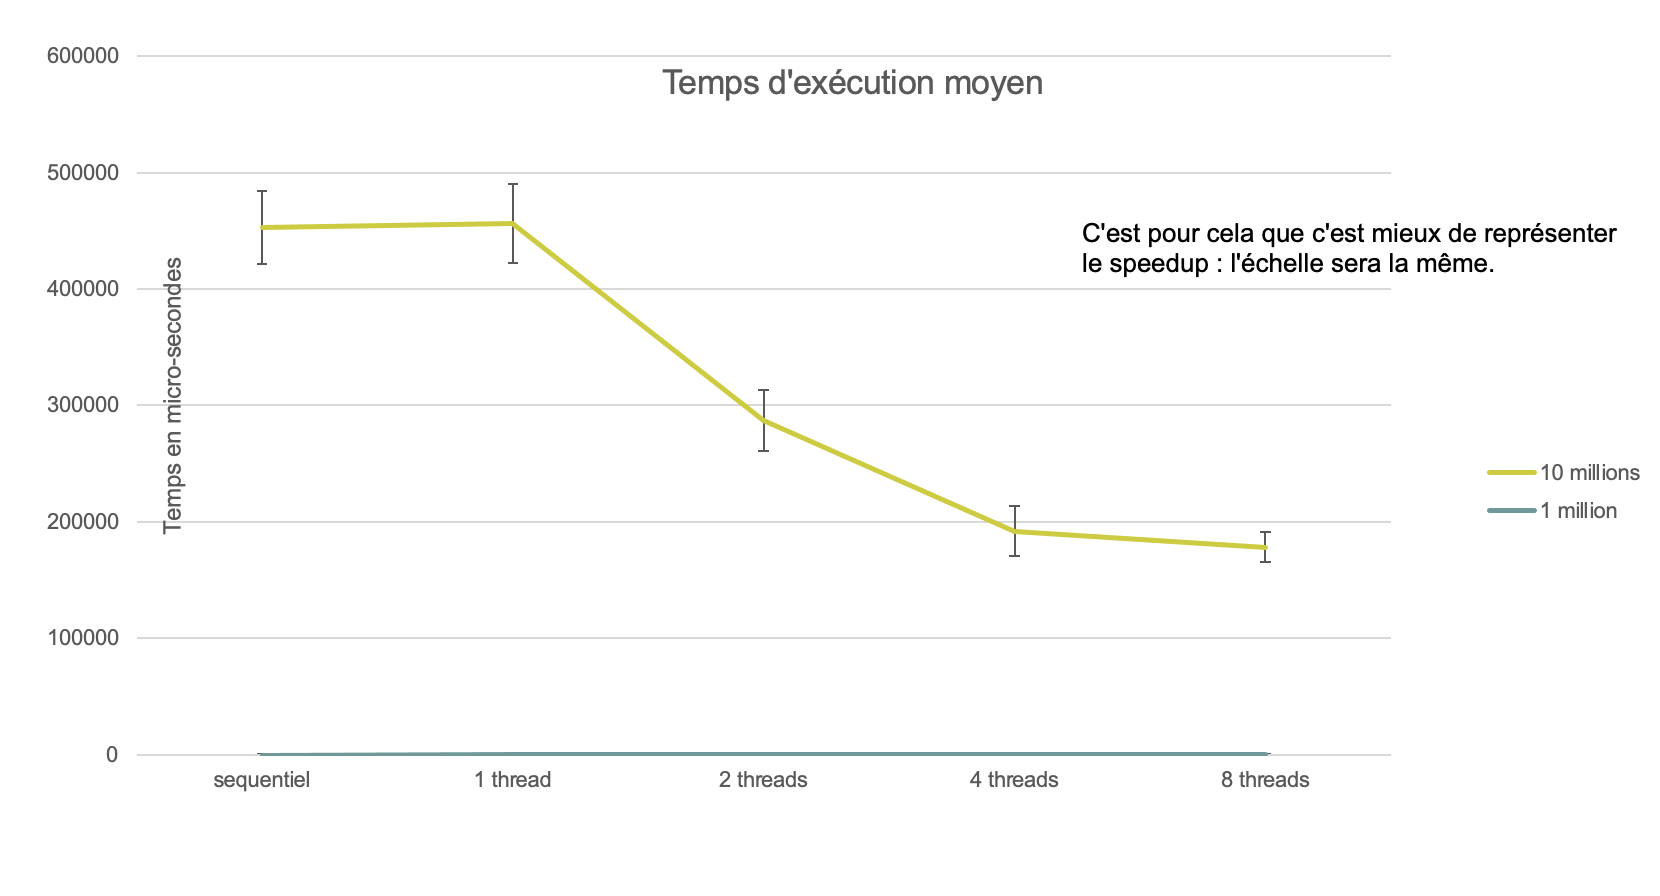
\includegraphics[scale=0.3]{figures/fig}
\caption{Temps d'exécution pour le tri d'un vecteur de ... éléments.}
\label{fig:index:uml}
\end{figure}


Sur la Figure~\ref{fig:t1} nous observons une grosse accélération pour 4 threads. L'accélération continue mais n'est pas aussi prononcée pour 8 et 16 threads, d'ailleurs nous voyons que la courbe se tasse. (la machine n'a que huit coeurs physiques et la création de plus de threads devrait se traduire par une degradation de perfs)

Les données concernant cette expérimentation sont fournis dans les fichiers ....

Vous pouvez donner des résultats dans des tables comme dans Table~\ref{tab:tempsMoyen}.

\begin{table}[ht]
\centering
\begin{tabular}{l|l|l}
Nb threads  & Taille vecteur & Temps moyen \mu s)\\ \hline \hline
1 & 1000 & ... \\ 
2 & 1000 & ... \\ 
4 & 1000 & ... \\ 
...  & ... & ... \\
...  & ... & ... 
\end{tabular}
\caption{Temps d'execution moyen pour ....}
\label{tab:tempsMoyen}
\end{table}

\subsection{Accélération dans le cas de vecteurs de taille moyenne}

Etude du speedup en fonction du nb de threads. Voir plus haut. Ne pas répéter les mêmes choses mais montrer le graphique et relever ce qui change.

\subsection{Accélération dans le cas de vecteurs de grande taille}

Etude du speedup en fonction du nb de threads. oir plus haut. Ne pas répéter les mêmes choses mais montrer le graphique et relever ce qui change.

\subsection{Accélération en fonction de la taille des vecteurs}

Graphique avec trois courbes, chaque courbe correspondant à une taille de vecteur. Axe Y : speedup, Axe X : nb de threads.

Commenter.

\section {Conclusion}



\end{document}
